\title{Experimental Laboratory 1\\Calibration of a load cell}
\author{
        Sergio M. Vanegas A.\\
        Francesco de Pas\\
                Department of Mathematics\\
        Polimi---Politecnico di Milano\\
        Milano, Italia
}
\date{\today}

\documentclass[12pt]{article}

\usepackage{amsmath}
\usepackage{graphicx}
\usepackage{siunitx}

\begin{document}
\maketitle

\begin{abstract}
        The second test case consists on the experimental calibration of a Load Cell (instrument for measuring Force). The load cell produces an electrical output (Voltage) which is approximately proportional to the applied force. In order to estimate the value a force with a load cell, it is necessary to determine the transfer function from voltage to newton \( V [volt] \rightarrow F [Newton] \). \cite{FL:02}
\end{abstract}

\section{Introduction}

        The transfer function is obtained by using mass samples whose weight force \( F^* \) is accurately known (see Figure~\ref{fig:sketch}); this operation is what's usually called calibration.

        \begin{figure}[!ht]
                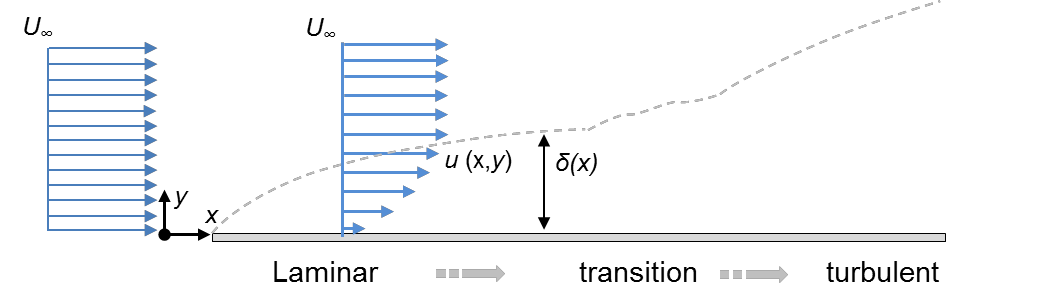
\includegraphics[width=0.75\textwidth]{Sketch.png}
                \centering
                \caption{Sketch of the Case}
                \label{fig:sketch}
        \end{figure}

        Each mass sample is applied to the load cell for a few seconds and the correspondent electrical output is recorded (the sampling frequency is \( f_s=100 \: H\!z \)). This produces a noisy signal like the one shown in Figure~.

        \begin{figure}[!ht]
                \includegraphics[width=0.75\textwidth]{Noise.png}
                \centering
                \caption{Noisy Load Cell signal example}
                \label{fig:noise}
        \end{figure}

        The voltage output histories and the corresponding values of the reference force, \( F^* \), are listed in the Table and provided in the form of MATLAB workspaces. Each workspace contains the vector of the readings in Volt (remember that the sampling frequency is \( f_s = 100 H\!z \)). In Table~\ref{tab:data}, the sign of F* is as presented in the sketch, namely, \( F^* > 0 \) when the force is directed upwards, and \( F^* < 0 \) when it is directed downwards.

        \begin{table}[!ht]
                \label{tab:data}
                \begin{tabular}{|cc|cc|}
                        \hline
                        \textbf{TestID} & \( \pmb{F^* \: \left[ N \right]} \) & \textbf{TestID} & \( \pmb{F^* \: \left[ N \right]} \) \\ \hline
                        calibr01        & 0.000               & calibr09        & -5.598              \\
                        calibr02        & -0.314              & calibr10        & -10.501             \\
                        calibr03        & -0.411              & calibr11        & 0.126               \\
                        calibr04        & -0.695              & calibr12        & 1.097               \\
                        calibr05        & -0.891              & calibr13        & 2.078               \\
                        calibr06        & -1.186              & calibr14        & 4.039               \\
                        calibr07        & -1.676              & calibr15        & 8.942               \\
                        calibr08        & -2.656              & calibr16        & 13.845              \\ \hline
                \end{tabular}
                \centering
                \caption{Reference Forces}
        \end{table}

        The main objective of the laboratory is to determine the transfer function for the load cell, and estimate the uncertainty of the instrument. For that purpose, the remainder of the report is organized as follows: Section~\ref{sec:stabilized_signal} graphically stimates the acquisition time required in order to get a stabilized measure out of an accumulating averaged voltage signal, and then provides the stabilized voltage value for each test case; Section~\ref{sec:lin_regression} performs a linear regression over the averaged voltage measure in function of the reference force; Section~\ref{sec:uncertainty} provides an approximation of the uncertainty we can expect from using the coefficients obtained in Section~\ref{sec:lin_regression} to estimate the value of the measured force in function of the averaged voltage signal; finally, Section~\ref{sec:resolution} provides an approximation of the resolution of the load cell based on the measured data from the test cases.

\section{Stabilized voltage measurement} \label{sec:stabilized_signal}

        \begin{figure}[!ht]
                \includegraphics[width=0.75\textwidth]{Averaged_Data.png}
                \centering
                \caption{Accumulated averaged data over time (normalized)}
                \label{fig:averaged}
        \end{figure}

        Following the guidelines, we proceeded to calculate the accumulated average of the sensor signal over time. Additionally, we normalized the difference between each partial average and the final one by this last value and plotted the square of this quantity, which is the signal we can observe on Figure~\ref{fig:averaged}. We can observe how the power of the error decreases by 3 orders of magnitude (at the very least) by the 10 second mark, turning it into a convenient criterion to start considerating the averaged measure as valid.

        Nevertheless, as a countermeasure to overfitting (and considered the data had already been gathered anyway), we decided to extract the median of each accumulated average after the 10 second mark and use it as the final measure.

\section{Linear regression} \label{sec:lin_regression}

        \begin{figure}[!ht]
                \includegraphics[width=0.75\textwidth]{Fitting.png}
                \centering
                \caption{Data linear regression}
                \label{fig:regression}
        \end{figure}

        After extracting the averaged measure, we proceeded to perform a linear regression on the data as a function of the reference applied force. The resulting formula corresponds to the one in Equation~\ref{eq:regression}.

        \begin{equation} \label{eq:regression}
                \mu_{V_0} = m F^{*} + b = (\SI{-4.077e-4}{\volt\per\newton}) F^{*} + (\SI{-2.901e-5}{\volt})
        \end{equation}

\section{Uncertainty estimation} \label{sec:uncertainty}

        Considering the random nature of the measurement process, we had to calculate the uncertainty \( U \) associated to the estimated force \( \widetilde{F} = \frac{V_0 - b}{m} \). For that purpose, we followed 2 different approaches:

        \begin{enumerate}
                \item Set \( U \) as the maximum absolute difference between \( \widetilde{F} \) and \( F^{*} \) for all the 16 calibration cases.
                \item Set \( U \) as a function of the confidence intervals for a perfect Gaussian PDF (\( 95\% \) confidence).
        \end{enumerate}

        The resulting uncertainties can be seen in Equation~\ref{eq:uncertainty_1} and Equation~\ref{eq:uncertainty_2} respectively.

        \begin{equation} \label{eq:uncertainty_1}
                U_1 = \sup_{i \in \{1,...,16\}} \left| \frac{V_i - b}{m} - F^* \right| = \SI{1.381e-2}{\newton}
        \end{equation}

        \begin{equation} \label{eq:uncertainty_2}
                U_2 = 2 \bar{S}_F = 2 \sqrt{\frac{1}{N-2} \sum_{i = 1}^{16}{\left(\frac{V_i - b}{m} - F\right)^2}} = \SI{1.179e-2}{\newton}
        \end{equation}

\section{Resolution estimation} \label{sec:resolution}

        Finally, we estimated the sensor's voltage resolution by ordering each measuring sequence and extraction the global minimum variation, which ended up being \( \SI{6.593e-6}{\volt} \). Then, making use of the linear regression coefficients calculated beforehand, we obtained the expression in Equation~\ref{eq:resolution} for the sensor's force resolution.

        \begin{equation} \label{eq:resolution}
                \Delta F = \inf_{\left\{ V_1, V_2 \right\}} \left| \frac{V_1 - b}{m} - \frac{V_2 - b}{m} \right| = \left| \frac{\Delta V}{m} \right| = \SI{1.617e-2}{\newton}
        \end{equation}

\bibliographystyle{abbrv}
\bibliography{main}

\end{document}
